\chapter{Introduction}

\textit{This chapter starts by presenting background and motivation on doing this thesis project. Afterwards, the problem statement and thesis' goals will be explained. Explanations on our contributions to the state-of-the-art will continue this chapter. This chapter will be closed by description of thesis' outline.}

\section{Need for Self-Sovereign Identity}
Hardly anyone can live without having their identity. Identity is the one that defines who we are, something which helps to describe the uniqueness of everyone.
Identity's role in our daily life is unquestionable. Society requires identity systems to enable identity-requiring transactions at scale, allowing procedures that require the formal asking and answering of identity queries in place, allowing millions of transactions to occur.
In modern society, identity is commonly related to social security cards, driver's licenses, and other state-issued credentials. Centralized controlled by the government is the definition of these elements.

Along with the rise of the digital age, identity also redefines itself. Identity in the digital world, can be referred as digital identity, is split into multiple domains. Our Facebook identity does not correlate directly to our Twitter identity or to most other domains. Digital identities are scattered, vary from one Internet domain to another. Scattered identities which locked to multiple entities leads to a problem where users are helpless in front of an authority who can deny their identity or even confirm a false identity. This phenomenon ignites a problem where users are not in control of their identity.
There's no clear construction and agreement on how to build the digital identity which usable across platforms. This is an unfortunate thing since lack of digital identity also limits the development and delivery of efficient, secure, digital-based economy and society \cite{blueprint}. The failure to solved the digital identity problem issue even looks a bit strange since we already have \textit{public key cryptography} since 1984, introduced by Chaum \cite{chaum}, which enable secure communication between parties without the hassle of key distribution problem and also provide valid digital signatures. Using public key cryptography, anyone who wants to send any message to a recipient needs to encrypt their message using the recipient's public key. Afterwards, the recipient can read the message after decrypting the received message using its private key.

To fix the scattered identity issue, a solution was proposed: one should be able to store their encrypted data in their own devices or in their own preferred service. To use the data, a service has to ask the data owner for the private key which will be used to decrypt the data. Using this concept, everyone has to keep their secret keys secure and solely in their possession.
A centralized storage of private keys is out of question since it will be a honeypot for cyber attacks. Simply put, keeping secret keys secure is the cardinal problem to solve here.


All problems mentioned above leads to a thinking, identity and secure key storage need to be solved in a decentralized manner.
In 2012, a new concept called \textit{self-sovereign identity} (SSI) arise \cite{moxytongue}.
Self-sovereign identity is a decentralized identity concept which capable of authenticating statements, without any central organization, point-of-failure or any possibility of data tracking \cite{pouwelse}. Self-sovereign identity will be able to give users full control over their identity. In simple words, users can store their identity data on their devices, and decide whether to give access to anyone who is willing to use it or not. In addition, there will be no need for a centralized storage since each user database is distributed among themselves. A high possibility to get this concept popular is also present with the introduction of the European Union General Data Protection Regulation \cite{eur-lex}.

At the end of 2017, Johan Pouwelse and Martijn de Vos proposed an SSI design which focused on data protection \cite{pouwelse}.
Data protection itself is related to securing data against unauthorized access \cite{data_protection_scheme}.
Their proposal is described by a concept where the user data are encrypted and never leave the device/domain. Any operation which requires the data, such as authentication, will require symmetric encryption on the encrypted data. This encrypted data should be securely protected and the domain should be trustworthy. In addition, the key used to encrypt and decrypt data should be kept securely.

The most common way to store the key is by using a \textit{non volatile memory} (NVM). NVM is a type of computer memory that keep intact its information even after turned off. An example of a product which implements this approach is the debit card. It uses its chip to store information. Unfortunately, this NVM is prone to physical attack. Since the key is permanently stored in the memory, an attacker can use some technique to clone the memory, such as \textit{microprobing} \cite{skorobogatov_2011}.  An attacker may also use a side channel information to retrieve any information about the key. There are numerous other techniques for this kind of attack. This attack can be even worse if someone that knows the system design is involved. Due to this problem, more secure, tamper-evident, tamper-proof solutions need to be presented.

\section{Rise of PUF as a Security Solution}
\label{ris_puf}
In 2001, Physical Unclonable Function (PUF) comes in handy as an inexpensive and yet effective security solution to overcome the mentioned problem above by a different way of generating and processing secret keys in security hardware. It was introduced by Pappu \cite{Pappu2026}. Unlike cryptographic algorithm security which usually relies on a hard-to-solve mathematical problem, PUF idea stems from using hardware features designed to utilize the physical random nanoscale disarray phenomena \cite{retrospective}. These disarray phenomena can be used as a derivation of keys without having to keep any security-critical information explicitly. This physical randomness is unclonable, even by the original manufacturer due to manufacturing process variations. Furthermore, since the secrets can only be produced when the PUF device is turned on, active manipulation of circuit structure will cause dysfunction of challenge-response mechanism and destroy the secret.

Related to self-sovereign identity concept, \cite{pouwelse} present an idea to use PUF and biometric-based authentication to securely protect the data in the self-sovereign identity. Figure \ref{fig:trust-creation} shows the detailed technology stack in their trust creation proposal on how to build trust in the blockchain era.

\begin{figure}[tph!]
    \centerline{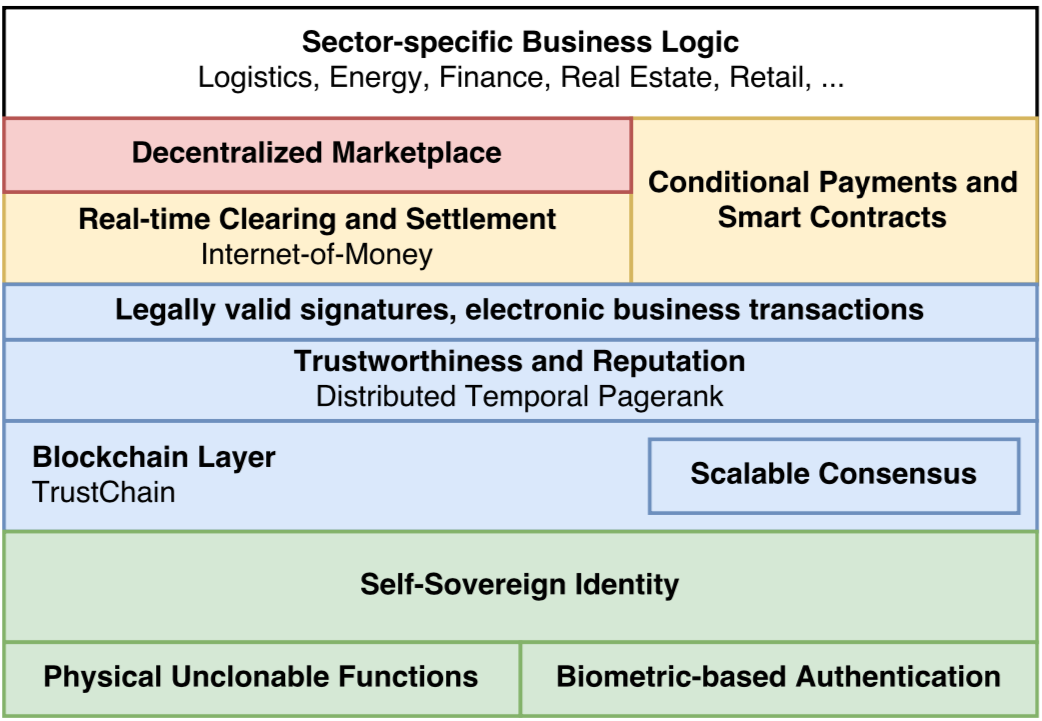
\includegraphics[width={0.8\textwidth}]{images/stack_ssi}}
    \caption{Detailed technology portfolio for trust creation in the blockchain age \cite{pouwelse}. As shown in the bottom of this figure, Physical Unclonable Functions and biometric-based authentication are utilized to secure the self-sovereign identity.}
    \label{fig:trust-creation}
\end{figure}

An example of PUF type is SRAM PUF. SRAM, stands for \textit{static random-access memory}, is a type of semiconductor memory that uses bistable latching circuitry (flip-flop) to store each bit. When a static RAM (SRAM) is turned on, the memory cells have undefined states \cite{tuyls_2010}. The initialized values on the memory cells are also random and unique to each SRAM. Based on these properties, SRAM is considered as a reasonable candidate for PUF. The value of these bits itself is determined by the SRAM cell which consists of two cross-coupled inverters along with two access transistors. This concept was first introduced by Guajardo and Holcomb in 2007 \cite{guajardo_kumar_schrijen_tuyls}. In order for SRAM to be used as a cryptographic security key, SRAM PUFs need to have certain characteristics such as the key generated by every SRAM should be reliable and unique. Reliable means the generated key should always be consistent, while unique refers to there should be no correlation between one device or another.
Unfortunately, SRAM PUF is also problematic since it contains noise in its bit value. To handle the noise, error correction code is usually utilized.

% \chapter{\chapterThree}
% \label{chp:3}
\section{Problem Statement}


Since introduced by Guajardo and Holcomb in 2007, there have been many innovations in SRAM PUF field. A simple patent search using patents.google.com with query 'sram; puf' results in 546 results \cite{google_patents}. The number of articles in \seqsplit{scholar.google.com} also exhibit a high occurrences, shown 2,120 articles (citations and patents are not included) \cite{google_scholar}.
Even though these facts indicate a promising future for this concept, one also should notice that current state-of-the-art in this field mostly consists of one-off prototypes or specific proprietary implementations.
To get an SRAM PUF product from the market, one has to order a specific request from a company. For example, Intrinsic-ID, one of the main leaders in SRAM PUF technology, has a software-based solution which able to generate unique keys and identities for nearly all microcontrollers without a need for security-dedicated silicon \cite{broadkey}. Even though this solution exists and seems easy to use, unfortunately, they don't say specifically how much will it cost to use this solution.
They also have another solution for SRAM PUF which is focused on hardware IP (and supporting software/firmware) to enable designers to implement PUFs within their design. This solution has a high possibility to obstruct a small company or a single user to use their solution since usually this type of product are intended to use with an expensive contract. Similar to the software-based solution they offer, they also don't put the explicit price to use this product. An example of a product that uses this solution is FPGA Microsemi Polarfire \cite{polarfire}.

The SRAM PUF field lacks an Arduino, Linux, or GCC type of open reference implementation. A quick lookup in Github shows that there's no extensive open source project related to SRAM PUF there. There are projects corresponding to PUF concepts, but most of them also only delve into a simulation.
The communities seem to haven't established a wide agreement on which approach yields the strongest security properties.

An additional issue that we would like to address is SRAM PUF's application. As mentioned in Chapter 1, the importance of securing key and user's data is getting higher, especially with the introduction of self-sovereign identity. There are already many SRAM PUF applications published, but sadly, there isn't any example working project that tries to integrate SRAM PUF in self-sovereign identity concept. Most PUF applications are designed for authentication \cite{Tuyls2007} \cite{delvaux} \cite{Suh:2007:PUF:1278480.1278484} \cite{10.1007/978-3-642-04474-8_22} \cite{10.1007/978-3-642-10838-9_22} \cite{10.1007/978-3-319-29078-2_5}
and generating cryptographic keys \cite{Suh:2007:PUF:1278480.1278484} \cite{10.1007/978-3-642-33027-8_18}.

Based on these facts, we believe the next challenge for this field is to discover a common approach. The field needs to move beyond isolated single-person projects and single-company approaches towards a mature and sharing ecosystem. The field SRAM PUF requires a single implementation which is continuously improved upon for many years to come and is supported by the majority of the academic and commercial parties.
Furthermore, we also try to initiate an attempt of integration between PUF and self-sovereign identity by providing a scheme to protect user's data and key. This project will be useful in the process of self-sovereign identity development.

To understand our intention in this thesis better, this thesis' problem statement is presented here. The problem statement of this thesis is:

\begin{adjustwidth}{1cm}{1cm}
		\textit{How to develop an open source secure data protection and key storage scheme using off-the-shelf SRAM component and software-based SRAM PUF technology?}
		% \textit{How to develop an open source secure data protection and key storage scheme using off-the-shelf SRAM component based on SRAM PUF technology?}
    % \textit{How to develop a secure software-only SRAM PUF-based data protection and key storage scheme using off-the-shelf SRAM while providing a mature and sharing ecosystem for continuous SRAM PUF development?}
\end{adjustwidth}

Derived from the problem statement, there are two goals defined in this thesis. The first goal is to devise a secure data protection and key storage scheme based on SRAM PUF technology. The data and the key protected by the scheme has to be safe even though the PUF device is lost. Moreover, the scheme should work using off-the-shelf SRAM. This sub-goal leads us to another question, can we build SRAM PUF using off-the-shelf SRAM? If it is possible, what characteristics need to be fulfilled by off-the-shelf SRAM to be eligible as a PUF candidate?
In addition, the constructed SRAM PUF has to work without any hardware design, or in other words, software-based construction. The data protection and key storage functions inside the scheme will be helpful in addressing the problem of self-sovereign identity and keeping the secret key.
The next goal is to create a sharing ecosystem for the evolution of our data protection and key storage scheme. The ecosystem should be easily accessed and understood to encourage the academics and commercial parties to use and develop the ecosystem together. The easiest step to achieve this goal is by making our thesis as an open source project.


\section{Contributions}
In our work, we strongly believe in open source idea and communities involvement when developing a system. Combined with the problems and potential of SRAM PUF mentioned before,
% and also driven by passions, willing to learn, and extensive brainstorming,
this thesis generates several additions into the state of the art of SRAM PUF knowledge. This thesis' contributions are explained below:
\begin{itemize}
    \item \textit{The first open project on software-based SRAM PUF using off-the-shelf SRAM.}
    % This is the first open project on software-based SRAM PUF.
    % The project can be found on a Github repository \cite{repository}.
    This software-based SRAM PUF project consists of Arduino codes and python codes and can be found on a Github repository \cite{repository}. It provides the off-the-shelf SRAM testing, enrollment and reconstruction mechanism which can be utilized to develop other applications. The testing part can be utilized to check whether an SRAM is capable to be a PUF root-of-trust or not. The enrollment stage will generate the helper data and the challenge which stored on a microSD connected to Arduino. The reconstruction part can generate a PUF-generated key based on the challenge and the helper data. In our construction, the selected off-the-shelf SRAM is Cypress CY62256NLL. We also tested another type of SRAM called Microchip 23LC1024 but we abandoned it due to insufficient results to be eligible as a PUF candidate. The enrollment stage also requires a bit selection algorithm called data remanence analysis. In the experiment part, there is another bit selection algorithm tested named neighbor analysis. This method is not selected due to worse performance than data remanence analysis.
    \item \textit{Procedure to develop an SRAM PUF-based application using any off-the-shelf SRAM.} The procedure consists of three main steps. First, one should be test the off-the-shelf SRAM quality to be a PUF component. If passed, the procedure continues to the next step which consists of enrollment and reconstruction mechanism which will be able to create a PUF-generated key. Last, using the PUF-generated key, one can develop any PUF-based application.
    % Based on our SRAM PUF construction, we also come up with an idea on how to develop an SRAM PUF-based application
    \item \textit{A scheme to enable secure data protection and key storage using off-the-shelf SRAM and software-based SRAM PUF.} This scheme is influenced by multi-factor authentication. Using a combination of the PUF-generated key and user's password, a derived key is produced and utilized as the final key to protecting user's data or/and user's key.
    % \item \textit{An open ecosystem to develop SRAM PUF using off-the-shelf SRAM.} The ecosystem consists of source code (Arduino and python code) and recommendations on how to test a possible SRAM candidate that might be used as an SRAM PUF. Using the system, we present testing results of two off-the-shelf SRAMs; Microchip 23LC1024 and Cypress CY62256NLL. Both SRAMs are tested on voltage variation and time interval between enrollment testing. The system also provides a bit selection algorithm; data remanence. This algorithm is also tested on these two SRAMs along with another bit selection algorithm, neighbor stability analysis. Neighbor stability analysis is not included in the final version of the project due to worse performance compared to data remanence analysis.
    \item \textit{A concept to devise numerous CRPs using SRAM PUF.} One of SRAM PUF weaknesses is the limitation of possible challenge-response pairs. We propose to use a set of bit locations as the challenge since when using this concept, the number of possible pairs is the permutation of total bit locations over the required number of bit locations. The total possible CRPs using this concept is a significant large number which can be bigger than the total number of atom in earth.
    % \item \textit{A concept to devise a strong PUF using SRAM PUF.} Normally, SRAM PUF is considered a weak PUF due to the limitation of possible challenge-response pairs. We propose to use a set of bit locations as the challenge since when using this concept, the number of possible pairs is the permutation of total bit locations over the required number of bit locations. The total possible CRPs using this concept is a significant large number which may lead to a \textit{strong PUF} definition.
\end{itemize}


\section{Outlines}
After explaining a brief review of SRAM's potentials and problems, problem statement and our contributions in this chapter,
Chapter \ref{chp:2} continues with an overview of security, cryptography, symmetric encryption, key derivation function and multi-factor authentication. Explanations of PUF and SRAM PUF are also presented in that chapter. Chapter \ref{chp:4} describes our proposed SRAM PUF development system, our idea on how to create numerous CRPs using SRAM PUF, and a scheme to enable secure data protection and key storage using SRAM PUF. Chapter \ref{chp:5} shows our implementation, experiments and results. Last chapter, Chapter \ref{chp:6}, summarizes this thesis and also gives our view on possible improvements on this project.
